% This file was converted to LaTeX by Writer2LaTeX ver. 1.9.9
% see http://writer2latex.sourceforge.net for more info
\documentclass{article}
\usepackage{calc,amsmath,amssymb,amsfonts,fontspec,xeCJK}
\usepackage{polyglossia}
\usepackage[style=authoryear-ibid,backend=biber]{biblatex}
\usepackage{graphicx,tikz}
\setdefaultlanguage[variant=british]{english}
\author{Changyang Li (LUT)}
\date{2026-01-09}
\begin{document}
 
\includegraphics[width=1.9807in,height=0.8543in]{a3BK10A6300Exercise1ReportTemplate-img001.png} 


\bigskip


\bigskip


\bigskip


\bigskip


\bigskip


\bigskip


\bigskip

Exercise 1

BK10A6300 Engineering Design


\bigskip


\bigskip


\bigskip


\bigskip

Lappeenranta–Lahti University of Technology LUT

2026

Author 1’s first name and last name

Author 2’s first name and last name

Author 3’s first name and last name

Author 4’s first name and last name


\bigskip

Examiner(s): Changyang Li

\clearpage\clearpage

Table of contents

You probably need to create a new “table of content” by clicking “Reference” – “Table of Contents”. If needed, change
the font and size to match other text in this template.


\bigskip


\bigskip


\bigskip

\clearpage\section{Introduction}
Write how your group work together in this exercise 1 (50 words max)

\subsection{Background information}
Write which reactor is chosen, search the latest figure about the reactor, and put one figure here. The figure must have
the caption, please check appendix 3 in this template. Please include at least 2 references from the journal papers.
(100 words max)


\bigskip

\subsection{Selected activities’ introduction}
Use the following figure to show which activities are selected. You need to replace it with the ones that you selected.

\begin{tikzpicture}
\end{tikzpicture}


Then for each task, including at least the following information:

\begin{enumerate}
\item at least 2 references from the journal papers for each activity
\item one figure of the component
\item parameters of the component, such as length/width/height/diameter/mass/density/material, etc…
\item what exactly is the activity. For example, if it is inspection, what will be inspected. If it is transportation,
what is the initial location and final destination, and through which method, vertically or horizontally, or both. If
it is cutting, what are the cutting method, etc…
\end{enumerate}
(around 200 words / activity)


\bigskip

\clearpage\section{Task 1}
This task 1 includes roadmap, implementation plan, and engineering bill of materials.

\subsection{Roadmap}
You need to save the MS project as a single PDF file first, it does not need to be A4 size, it can be in different
layout, and in the end of the exercise 1, you need to merge this roadmap to this main PDF file. Please do not use
screenshot, which will decrease the resolution, and the text is too small to evaluate.


\bigskip

\subsection{Implementation plan}
You can make the implementation plan in excel, then save it as PDF, then merge it with the main PDF file in the same way
as the roadmap


\bigskip

\subsection{Engineering Bill of Materials}
Start with the selected activities, machine types, and specific machine, modify the chart below, and change the size of
the font and layout to make it easier to read. Short explanations:

Activity: should be the same as the one you selected in section 1.2.

Machine type: it can also be seen as category, such as crane, spider robot, drone, etc…

Specific machine: the exact code/model of the machine, such as KUKA titan 1000, this must be a specific machine.

\begin{tikzpicture}
\path (0,4.444) rectangle (15.500,0);
node[inner sep=0pt] at (7.750,2.222)
{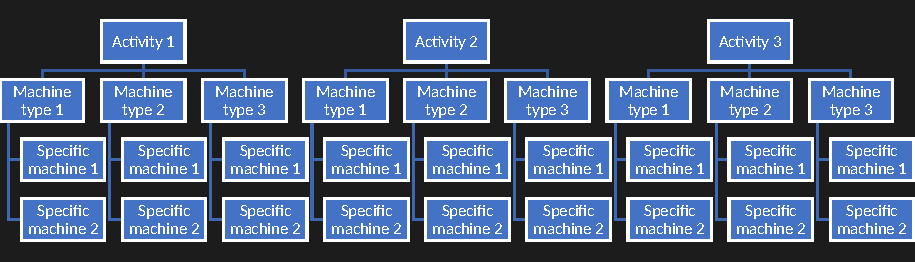
\includegraphics[width=6.1024in,height=1.7496in]{a3BK10A6300Exercise1ReportTemplate-img002.pdf}};
\end{tikzpicture}


Then fill in the EBOM sheet in the given excel form, and save it as PDF, merge it with the main PDF file in the same way
as the roadmap.


\bigskip

\clearpage\section{Task 2}
The task 2 includes the datasheet, system requirement document, and the context definition document. Please make sure
the code of each product in different document is unified.


\bigskip

\subsection{Datasheet}
Briefly introduce how you distribute the work here. Please note, each group member must be involved in this task, such
as responsible for some product search. Once this is finished, save each product’s datasheet as single PDF, then merge
it with the main PDF file. Please note, one product/page, and the resolution of the page must be high enough to read
easily.


\bigskip

\subsection{System requirements document (SRD)}
Briefly introduce how you distribute the work here. Please note, each group member must be involved in this task, such
as responsible for some product search. Save the sheet as PDF, then merge it with the main PDF file. Please note, one
product/page, and the resolution of the page must be high enough to read easily.


\bigskip

\subsection{Context definition document (CDD)}
Briefly introduce how you distribute the work here. Please note, each group member must be involved in this task, such
as responsible for some product search. Save the sheet as PDF, then merge it with the main PDF file. Please note, one
product/page, and the resolution of the page must be high enough to read easily.

\clearpage\section{Conclusions}
In case you have other things you want to include here, please write here.


\bigskip

\clearpage\section{References}

\bigskip


\bigskip

Hirsjärvi, S., Remes, P. \& Sajavaara, P. 2009. Tutki ja kirjoita. 15th ed. Helsinki, Tammi.

Stratton, C. R. 1976. Needs assessment for communication system design. Journal of Technical Writing and Communication.
Vol. 6, no. 2, pp. 135–144.

Virtanen, V. 2011. Esimerkkilähteen otsikko. Lappeenranta–Lahti University of Technology LUT. Accessed 1 January 2018.
Available at the LUT Academic Library


\bigskip

Note: More information on referencing is available in Appendix 2.

\clearpage

Delete everything starting from this page

Appendix 1. Text processing and layout in a thesis 

Good text processing skills make writing your final thesis and using this template easier. Therefore, you should make
sure you have the sufficient basic skills to edit long documents with text processing software before you start. This
involves applying the styles, understanding automatic referencing and knowing how to divide your text into sections. 


\bigskip

The essential thing is to understand the following basics of Word:

\begin{itemize}
\item Do not modify your layout by adding consecutive spaces or line breaks. If you need to press Enter or the space bar
more than once, you are probably doing something wrong. When you want to start a new paragraph, press Enter once at the
end of the sentence and use styles to create a space between the paragraphs.
\item Do not do numbering manually. Word has efficient automatised tools for this. Section numbering and page numbering
are applied in this template. They keep the numbers in the right order even if you modify, add or remove information.
\item Do not add hyphenation at the end of a line manually. Word’s automatic hyphenation tool can be used in this
template. If you need to add more hyphens, select manual hyphenation in Word. The automatic hyphenation is usually
turned off, but you can activate it yourself.
\end{itemize}

\bigskip

Line spacing, font, margins, alignment, page numbering and headings 


\bigskip

Official layout guidelines state that the line spacing should be 1.5 except for the abstract and possible direct
citations, where the spacing is 1. You can choose from two fonts: Times New Roman (12 pt) or Arial (11 pt). This
template has been written in Times New Roman 12 pt (Style LUT Normal). Leave an empty line between paragraphs. Also
leave an empty line after tables and figures.


\bigskip

Leave the following margins:

•\ \ top and left 35 mm

•\ \ bottom and right 20 mm. 


\bigskip

The page number of the title page is 1, but the page numbering should not be visible before the first page of the table
of contents. Place the page numbers at the top of the page, either centred or in the right-hand corner. Page numbering
ends on the final page of the reference list: appendices do not have page numbers unless the appendix is multiple
pages. 


\bigskip

Always use heading styles in your headings (LUT Heading 1, LUT Heading 2, LUT Heading 3). Always place chapter headings
(LUT Heading 1) on a fresh page. If you add large figures or tables, remember to check that the empty space after the
figure or image covers no more than 20\% of the page. 


\bigskip

The heading numbering starts from the introduction and continues consecutively. Do not place a period after the heading
number. Do not number the heading of the reference list at the end of the thesis. 


\bigskip

The thesis should include no more than three heading levels, and the headings should progress in a logical order (first
LUT Heading 1, then LUT Heading 2, etc.). If you need even more detailed subheadings, do not number them, and leave
them out of the table of contents. Concise headings that describe the text sufficiently are the best. You can use
question marks or exclamation marks, but do not add a period if the heading is a regular sentence. 


\bigskip

A heading cannot be followed by a heading. Always write something between them. For instance, there must be text between
headings 1 and 1.1. 


\bigskip

Lists are a good way to express things clearly. Use the same type of bullet or symbol in lists throughout your thesis. A
section should never end in a list. There should always be two or three sentences after a list. 

\clearpage

Appendix 2. References 

The text must include references to the sources you use. LUT University applies the Harvard referencing style, also
called the author-date style with in-text referencing and a detailed reference list at the end. 


\bigskip

The purpose of a reference is to provide sufficient information on a source used in the study, allowing the reader to
consult the original source for further information. The reference enables the reader to find detailed information on
the source easily in the list of references. You should refer to the original and most recent sources. If no new
studies have been published on the topic in question, also older ones may be used.


\bigskip

Referring to a source means that you explain the contents of the source material in your own words. Direct citations, on
the other hand, are placed in parentheses (“ ”). Plagiarism or using another person’s original material without
appropriate referencing is not allowed.


\bigskip


\bigskip

Referencing technique


\bigskip

In the Harvard system, the citation is placed in parentheses directly in the text to indicate the passage that has been
cited from another source. Place the citation before the period that ends the sentence when it refers only to the
sentence in question (Kaasinen et al. 2020, 173–174). If you are referring to more than that one sentence, place the
citation after the paragraph like a sentence of its own. In such cases, add a period at the end of the citation.
(Kaasinen et al. 2020, 174.)


\bigskip

Typically, the citation mentions the author (the last name is sufficient, unless authors of several sources have the
same last name), the publication year and the page number. Please note that the author does not always have to be a
person, but it may also be an organisation, for instance. If the source does not mention who the author is, the
reference should include the name of the publication instead of the author. (Nykänen 2002, 77.) The author (or the
title of the work) is very commonly mentioned as a part of a sentence: “According to a study conducted by Möttönen
(2007, 68), a pike is a fish”.


\bigskip

If the source has more than one author, they are all mentioned in the reference by their last name and separated with
the word ‘and’ or the symbol ‘\&’. Make later references to the same work with the first author’s last name and “et
al.” If you reference several works published by the same author in the same year, add lower-case letters (a, b, c…)
after the publication year to distinguish the sources. Use the same alphabetical organisation also in the list of
references.


\bigskip

There are several referencing and citation styles. It is essential to consistently use the same style throughout the
thesis. Examples and detailed instructions on referencing:

LUT Academic Library’s instructions on how to cite electronic documents

Aalto University citation guide 

Harvard referencing, University of Sheffield 

\clearpage

Appendix 3. Tables, figures, equations, numbers, symbols and abbreviations 

It is a good idea to illustrate your text with figures and tables. Figures and tables must have captions and consecutive
numbering. The captions of tables are placed above the table and those of figures below the figure. Refer to the
figures and tables in the text body, preferably before you introduce them, and align them with the text body. 


\bigskip

Remember to add alt text (alternative text) to your figures and tables to ensure accessibility. Alt text is read with a
designated reader and can be viewed even when the image cannot be displayed on the page. The MS Word text processing
software creates alt text automatically, but you should make sure it describes the object sufficiently and
understandably. You can modify the alt text by right-clicking on the figure or table.


\bigskip

Tables


\bigskip

Give your tables numbers and captions. Place the caption above the table, name its columns and mention the units
applied, as in Table 1 below. Avoid empty columns or rows. The recommended font size is 10.


\bigskip

Table 1. Sensor measurements

 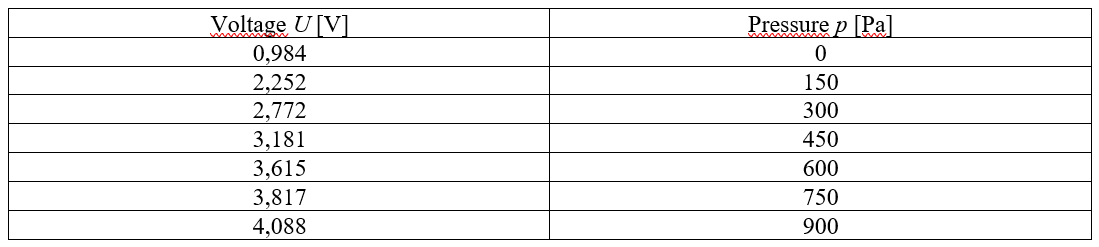
\includegraphics[width=6.102in,height=1.3717in]{a3BK10A6300Exercise1ReportTemplate-img003.png} 


\bigskip


\bigskip


\bigskip

Figures, charts, graphic elements


\bigskip

Images help illustrate your text. The text should contain a reference to the image (Figure 1). Number your figures and
place a caption underneath. You should use a software programme such as Excel or Matlab to draw charts. Charts should
be clear and easy to understand. Use a white background. A background grid is allowed if it does not make the figure
difficult to interpret. Variables and measurement points should be clearly visible, as in Figure 1. Name the axes and
their units. 


\bigskip

 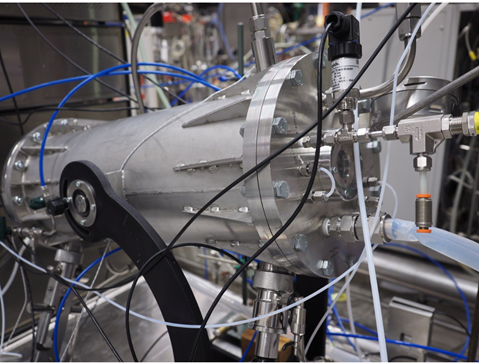
\includegraphics[width=3.1937in,height=2.4272in]{a3BK10A6300Exercise1ReportTemplate-img004.png} 

Figure 1. Gas fermentor (VTT 2020, LUT image bank).


\bigskip

Create as much of the figures yourself as you can. Use the same font as in the text body and equations. If you use
images created by someone else, remember to cite them correctly. Captions need to be in the same language as the text
body.


\bigskip

Do not end a paragraph in a figure or table. Add text underneath, such as comments on the figure. Large figures, tables,
long equations and other supporting material can be appended, if needed. 


\bigskip


\bigskip

Numbers, symbols and equations


\bigskip

Numbers in the text are usually approximations. Their accuracy depends on the observational error. Include only
significant figures in the results. Interim results should include at least two figures more to avoid round-off errors.
Present large and small figures in powers of ten 10ⁿ, where n should preferably be divisible by three.


\bigskip

Equations and other mathematical expressions must consist of standardised symbols if ones exist. You may use your own
symbols only there are no applicable standardised or established ones.


\bigskip

Explain the symbols in an equation when you use them for the first time. Write each equation clearly on its own line and
indent it. Number your equations consecutively or by paragraphs so that the number is in parentheses on the right side
of the equation and aligned to the right. You can refer to an equation only after you have presented it, with certain
exceptions, such as if the object you are referring to is far ahead. Example:


\bigskip

pv = RT\ \ \ \ \ \ \ \ \ \ (1)


\bigskip

where p is pressure [Pa], v is specific volume [m³/kg], R is the gas constant [J/kgK] and T is temperature [K].


\bigskip

When you write symbols in your thesis, do the following: 

\begin{itemize}
\item Write all variables in italics. 
\item Write subscripts upright unless there is a need to italicise them. Write abbreviated subscripts and numerals e.g.
as follows: $\Delta $$\sigma $w, $\sigma $1, $\sigma $min. For instance, in the summation  $\sum _i^{∞}x_i$ \ the
subscript needs to be italicised because it represents a running number i . 
\item If you wish to express change in e.g. pressure $\Delta $p, write $\Delta $ in a regular font. In some cases,
$\Delta $ may also be a variable and should then be italicised. \  is the ratio of a circle’s circumference to its
diameter.  may be the pressure ratio.
\item Do not italicise mathematical operators such as sin x or lg y.
\item Distinguish absolute values as follows: ”variable\_=\_number\_unit”, with the exception of a percentage sign after
a numeral, e.g. a = 5.2 mm,  \ = 97.7\%.
\end{itemize}

\bigskip
\end{document}
